\documentclass[../../tesis_maestria]{subfiles}
\begin{document}

\section{El truco ``3-5''}\label{sec:3-5}


\begin{comment}%%%%%%%%%%%%%%%%%%%%%%%%%%%%%%%%%%%%%%%%%%%%%%%
El pop\'osito de esta secci\'on es probar el siguiente teorema:
\begin{thm}
  Sea $E/\QQ$ una curva el\'iptica semiestable. Entonces
  \[
    \rhot\;\;\text{es reducible}\quad\then\quad \rhoc\;\;\text{es irreducible}.
  \]
\end{thm}
Este teorema permite reducir STW a dos casos: podemos asumir que $\rhot$ es irreducible o que es $\rhoc$ irreducible. Para hacer esto necesitamos calcular propiedades espec\'ificas de dos curvas modulares: $X_0(15)$ y $X_0(50)$. Afortunadamente Birch tiene un informe extenso de los c\'alculos necesarios para estudiar $X_0(50)$. Entonces seremos expl\'itos con
la curva $X_0(15)$.
\end{comment}%%%%%%%%%%%%%%%%%%%%%

En esta secci\'on estudiamos las propiedades aritméticas de la curva elípítica $X_0(15)$ para probar:

\begin{thm}\label{thm:3-5trick}%%%%%%%%%%%%%%%%%%%%%%%%%%%%%%
	Sea $E/\QQ$ una curva elíptica. Si $\rhot$ y $\rhoc$ son reducibles, entonces $E$ es modular.
\end{thm}

Este teorema es la  primera parte de la estrategia que usó Wiles para poder reducir el problema de probar la modularidad de una representación $\bar{\rho}_{E,\l}$ a probar la modularidad de $\rhot$. Si $\rhot$ es irreducible, aplicamos el teorema de Langlands-Tunnell como vimos en la sección \ref{sec:langlands_tunnell}. Si $\rhot$ no es irreducible, Langlands-Tunnell no se puede aplicar, pero lo que dice el teorema \ref{thm:3-5trick} es que podemos asumir que $\rhoc$ es irreducible. Este nuevo dato nos va a permitir construir una familia de curvas elípticas, todas con la misma representación módulo 5, que contiene al menos una curva $E'$ cuya representación $\bar{\rho}_{E',3}$ es irreducible.

Para justificar esta nueva vía, necesitamos el teorema \ref{thm:3-5trick}. La estrategia de probarlo es parametrizar la familia de curvas elípticas tales que $\rhot$ y $\rhoc$ reducibles, con los cuatro puntos racionales de $X_0(15)$ no cuspidales, i.e. $Y_0(15)(\QQ)$. Cada punto corresponde a una clase de isomorfismo de curvas elípticas cuyos isomorfismos preservan un subgrupo cíclico de orden 15. Con esta descripción de las curvas elípticas con $\rhot$ y $\rhoc$ reducibles, es posible asociarles una forma primitiva en $S_2(\Gamma_0(50))$ y así probar la modularidad de esas curvas elípticas. 

El primer paso es probar:

\begin{lema}\label{prop:cyclesubgroupE}%%%%%%%%%%%%%%%%%%%%%%
	  Si $E$ es una curva el\'iptica sobre $\QQ$ tal que $\rhot$ y $\rhoc$ son reducibles, entonces $E(\ol{\QQ})$ contiene un subgrupo cíclico de orden 15 que es estable bajo la acción de $\GQ$.
\end{lema}

\begin{proof}
  Supongamos que $\rhot$ y $\rhoc$ son reducibles. Por definici\'on existen subespacios no triviales $V_3\subset E[3]$ y $V_5\subset E[5]$ que son invariantes bajo la acci\'on de $\GQ$. Recuerda que $\# E[N]=N^2$, entonces el orden de cualquier subgrupo divide a $N^2$, pero en este caso $N=3,5$. Por lo tanto cualquier subgrupo no-trivial de $E[3]$ (respectivamente $E[5]$) necesariamente es de orden 3 (respectivamente 5). En particular $V_i\cong \ZZ/i\ZZ$ para $i=3,5$ y sean $P_3$ un generador de $V_3$ y $P_5$ un generador de $V_5$. Por \'ultimo, como subgrupos de $E(\overline{\QQ})$, $V_3$ y $V_5$ tienen intersecci\'on trivial (porque los elementos distintos del neutro de $V_3$ tienen orden 3 y los de $V_5$ tienen orden 5).
  
  Ahora definimos $V=V_3+V_5=\{P+P'\in E(\overline{\QQ}) \mid P\in E[3],\; P'\in E[5]\}$. Claramente el orden de cada punto de $V$ divide a 15 pues $15(P+P')=5(3P)+3(5P')=3O+5O=O$, es decir $V\subset E[15]$. Por otro lado el punto $P_3+P_5$ es de orden exactamente 15 porque
  \[
    3(P_3+P_5)=3P_5\neq O \quad\mathrm{y}\quad 5(P_3+P_5)=5P_3=2P_3\neq O.
  \]
  Por lo tanto $V$ es un subgrupo de $E(\overline{\QQ})$ de orden 15.

  Por \'ultimo, $V$ es invariante bajo la acci\'on de $\GQ$. En efecto, sea $\sigma\in\GQ$ arbitrario, entonces
  \[
    (P+P')^{\sigma}=P^{\sigma}+P'^{\sigma}\in V_3+V_5=V
  \]
  ya que la $\GQ$-estabilidad de $V_3$ (respectivamente de $V_5$) implica que $P^{\sigma}\in V_3$ (respectivamente $P'^{\sigma}\in V_5$). Por lo tanto $E(\overline{\QQ})$ contiene un subgrupo de orden 15 estable bajo la acci\'on de $\GQ$.
\end{proof}

El siguiente paso es estudiar la categoría de curvas elípticas con un subgrupo cíclico de orden 15 distinguido. Más precisamente, los objetos son parejas $(E',C')$ donde $E'/\CC$ es una curva elíptica con un subgrupo cíclico $C'$ de $E(\ol{\QQ})$ de orden $N=15$. Los isomorfismos de esta categoría son isomorfismos $\varphi:E'\ra E''$ tales que $\varphi(C')= C''$ que definen una relación de equivalencia sobre estas parejas que denotamos por $(E',C')\sim(E'',C'')$. Al conjunto de clases de equivalencias lo denotamos $S_0(N)=\{[E',C']\}$. Si queremos restringir las curvas elípticas a curvas sobre algún subcampo $K$ de $\CC$, denotamos por $S_0(N)(K)$ al conjunto de clases de equivalencias $[E',C']$ donde $E'$ está definida sobre $K$ y $C'\subset E'(K)$.

Podemos hacer una primera reducción. Gracias al teorema de uniformización (cf. el teorema \ref{thm:unif}), para toda curva elíptica $E'/\CC$ existe un $\tau\in\HH$ tal que $E'\cong \CC/(\tau\ZZ\oplus\ZZ)$ como grupos de Lie; denotamos $\Lambda_\tau:=\tau\ZZ\oplus\ZZ$ y  $E_\tau:=\CC/\Lambda_\tau$. Con esta notación tenemos el siguiente lema:

\begin{lema}\label{lema:espacio_moduli_Y_0(N)}
	Todo elemento $[E',C']\in S_0(N)$ es de la forma $[E_\tau,\gen{N^{-1}+\Lambda_\tau}]$ para alguna $\tau\in\HH$. Además, la función $\Psi:S_0(N)\ra Y_0(N)$ definido por $[E_\tau,\gen{N^{-1}+\Lambda_\tau}]\mapsto \tau\Gamma_0(N)\in Y_0(N)$ es una biyección.
\end{lema}

\begin{proof}
Sea $[E',C']\in S_0(N)$ y sea $Q\in C'$ un generador, en particular $Q$ es de orden $N$. Por el teorema de uniformización $E_\tau\cong E'$ para alguna $\tau$. Bajo este isomorfismo, $Q$ corresponde a un punto de $E_\tau$ que denotamos por
\[	
	Q=z_0+\Lambda_\tau\qquad(z_0\in\CC).
\]
Como $Q$ es de orden $N$, entonces $Nz_0\in\Lambda_\tau$ lo cual implica que existen $a,b\in\ZZ$ tales que $Nz_0=a\tau+b$. Como $\{1,\tau\}$ es una $\RR-$base de $\CC$, existen $\la,\mu\in\RR$ tales que $z_0=\la\tau+\mu$. Si igualamos ambas expresiones de $z_0$, obtenemos que $N\la=a$ y $N\mu=b$ y por lo tanto $\la,\mu\in\QQ$. De otra manera:
\[
	Q=\frac{\alpha\tau+\beta}{\gamma}+\Lambda_\tau\qquad(\alpha,\beta,\gamma\in\ZZ).
\]
Otra vez por el orden de $Q$, multiplicamos la ecuación anterior por $N$ y obtenemos: $N(\alpha\tau+\beta)/\gamma\in\Lambda_\tau$ y así $N\alpha/\gamma,N\beta/\gamma\in\ZZ$. Sin pérdida de generalidad podemos tomar $(\alpha,\beta,\gamma)=1$, entonces podemos concluir que $\gamma\mid N$. Por otro lado, si $\gamma<N$ entonces $\gamma Q=\alpha\tau+\beta+\Lambda_\tau=\Lambda_\tau$ lo cual contradice que $Q$ tiene orden $N$. Por lo tanto $\gamma=N$ y podemos asumir que existen $c,d\in\ZZ$ tales que
\[
	Q=\frac{c\tau+d}{N}+\Lambda_\tau\qquad(c,d,N)=1.
\]
Observe que si $t,t'\in\ZZ$ entonces la ecuación
\[
	\frac{(c+tN)\tau+(d+t'N)}{N}+\Lambda_\tau=
	\frac{c\tau+d}{N}+t\tau+t'+\Lambda_\tau=
	\frac{c\tau+d}{N}+\Lambda_\tau=Q
\]
implica que la elección de $c$ y $d$ depende solamente de sus clases módulo $N$.

Por las hipótesis sobre $c,d$ y $N$, existen $a,b,k\in\ZZ$ tales que $ad-bc+kN=1$ es decir, si denotamos
\[
	\sigma=\mat{a}{b}{c}{d}\in M_2(\ZZ),
\]
entonces bajo la proyección $\pi:M_2(\ZZ)\epi M_2(\ZZ/N\ZZ)$, tenemos que $\pi(\sigma)\in\SL_2(\ZZ/N\ZZ)$. Como la restricción $\pi:\SL_2(\ZZ)\ra\SL_2(\ZZ/N\ZZ)$ es sobreyectiva, toma $$\sigma'=\mat{a'}{b'}{c'}{d'}\in\SL_2(\ZZ)$$ tal que $\pi(\sigma')=\pi(\sigma)$. Por construcción, $c\equiv c'\Mod{N}$ y $d\equiv d'\Mod{N}$ entonces
$Q=(c'\tau+d')/N+\Lambda_{\tau}$.

Sea $\tau'\in\HH$ tal que
\begin{equation}\label{eq:def_de_matriz_sigma}
  \tau'=\sigma'\tau=\frac{a'\tau+b'}{c'\tau+d'}
\end{equation}
y denotamos al denominador por $m=c'\tau+d'$. Entonces $m\tau'=(a'\tau+b')$ y así
\begin{equation}\label{eq:reticulas_iguales}
	m\Lambda_{\tau'}=
	m(\tau'\ZZ\oplus\ZZ)=
	m\tau'\ZZ\oplus m\ZZ=
	(a'\tau+b')\ZZ\oplus(c'\tau+d')\ZZ.
\end{equation}

Es conocido que dos retículas $\omega_1\ZZ\oplus\omega_2\ZZ$ y $\omega'_1\ZZ\oplus\omega'_2\ZZ$, tales que $\Im(\omega_1/\omega_2),\Im(\omega'_1/\omega'_2)>0$, son iguales si $\omega_1/\omega_2,\omega'_1/\omega'_2\in\HH$ están en la misma órbita de la acción $\PSL_2(\ZZ)\act\HH$.\footnote{\label{foot:reticulas}Más precisamente, si $\mathcal{R}$ es el espacio de retículas, $\CC^*$ actúa por homotecias. Entonces $\omega_1\ZZ\oplus\omega_2\ZZ\mapsto \omega_1/\omega_2$ es una biyección $\mathcal{R}/\CC^*\ra\HH/\PSL_2(\ZZ)$ (cf. la proposición 3 de $\S2$ del capítulo VII de \cite{SerreACIA}). En particular tenemos que
\[
	\omega_1\ZZ\oplus\omega_2\ZZ=\omega'_1\ZZ\oplus\omega'_2\ZZ \quad\iff\quad
	\omega'_1=a\omega_1+b\omega_2,\;\;\omega'_2=c\omega_1+d\omega_2\quad\text{donde}\;\;\mat{a}{b}{c}{d}\in\SL_2(\ZZ)
\]} En este caso tenemos que $(a'\tau+b')\ZZ\oplus(c'\tau+d')\ZZ=\tau\ZZ\oplus\ZZ$ porque $(a'\tau+b')/(c'\tau+d')=\tau'=\sigma'(\tau)$ y así $\tau/1$ y $(a'\tau'+b')/(c'\tau'+d')$ están en la misma órbita. De \eqref{eq:reticulas_iguales} concluimos que $m\Lambda_{\tau'}=\Lambda_{\tau}$ y que
\[
	m\paren{\frac{1}{N}+\Lambda_{\tau'}}=\frac{c'\tau+d'}{N}+\Lambda_\tau=Q.
\]
Por lo tanto el homomorfismo $E_{\tau'}\ra E_\tau$ definido por $z+\Lambda_{\tau'}\mapsto mz+\Lambda_{\tau}$ es un isomorfismo\marginpar{\scriptsize{No sé si agregar una parte de retículas a la sección de curvas elípticas para justificar este isomorfismo}}. Si lo componemos con el isomorfismo $E_\tau\cong E'$ obtenemos un isomorfismo $f:E_{\tau'}\ra E'$ donde $f(N^{-1}+\Lambda_{\tau'})=Q$. De esta manera $f\big(\gen{N^{-1}+\Lambda_{\tau'}}\big)=\gen{Q}=C'$. Concluimos que $[E',C']=[E_{\tau'},\gen{N^{-1}+\Lambda_{\tau'}}]$ para alguna $\tau'\in\HH$.

Ahora demostramos la segunda parte del lema. Tenemos que probar que la función $\Psi:[E_\tau,\gen{N^{-1}+\Lambda_\tau}]\mapsto\tau\Gamma_0(N)$ cumple tres cosas:
\begin{enumerate}[label=\emph{\roman*})]

  \item $\Psi$ está bien definida.
  
  \-\;\;Si $[E_\tau,\gen{N^{-1}+\Lambda_\tau}]=[E_{\tau'},\gen{N^{-1}+\Lambda_{\tau'}}]$, entonces $\CC/\Lambda_\tau\cong\CC/\Lambda_{\tau'}$ y por lo tanto existe un $m\in\CC^*$ tal que $m\Lambda_\tau=\Lambda_{\tau'}$ (véase la nota de pie \ref{foot:reticulas}) y tal que $z+\Lambda_\tau\mapsto mz+\Lambda_{\tau'}$ induce el isomorfismo anterior. Como $\Lambda_\tau=\tau\ZZ\oplus\ZZ$, entonces la igualdad $m\Lambda_\tau=m\tau\ZZ\oplus m\ZZ=\tau'\ZZ\oplus\ZZ$ nos dice que existe un
\[
	\sigma=\mat{a}{b}{c}{d}\in\SL_2(\ZZ)
\]
tal que
\[
	m\tau=a\tau'+b\quad,\quad m=c\tau'+d
\]
o en particular $\sigma\tau'=\tau$; esto es otra vez por la nota de pie \ref{foot:reticulas}.

  \-\;\; Por otro lado sabemos que el isomorfismo $E_\tau\cong E_{\tau'}$ manda $N^{-1}+\Lambda_\tau$ en $\gen{N^{-1}+\Lambda_{\tau'}}$, es decir
\[
	m\paren{\frac{1}{N}+\Lambda_\tau}=\frac{c\tau'+d}{N}+\Lambda_{\tau'}=\frac{k}{N}+\Lambda_{\tau'}\quad (1\leq k< N)
\]
donde $(k,N)=1$ porque $k/N+\Lambda_{\tau'}$ es necesariamente de orden $N$. La ecuación anterior implica que
\[
	\frac{c}{N}\tau'+\frac{d-k}{N}\in\Lambda_{\tau'}\quad\then\quad N\mid c,\;\; N\mid d-k.
\]
Si $\delta$ fuese un factor común de $N$ y $d$, entonces $\delta\mid d-k$ implica que $\delta\mid k$ y así $\delta\mid(N,k)=1$. Por lo tanto $(N,d)=1$ y así deducimos que $c\equiv0\Mod{N}$ y $d\equiv1\Mod{N}$. Con esto concluimos que $\sigma\in\Gamma_0(N)$. Como $\sigma\tau'=\tau$, tenemos que $\tau\Gamma_0(N)=\tau'\Gamma_0(N)$ cuando $[E_\tau,\gen{N^{-1}+\Lambda_\tau}]=[E_{\tau'},\gen{N^{-1}+\Lambda_{\tau'}}]$ y por lo tanto la función $[E_\tau,\gen{N^{-1}+\Lambda_\tau}]\mapsto\tau\Gamma_0(N)$ está bien definida.

  \item $\Psi$ es inyectiva.
  
  \-\;\; Sean $\tau,\tau'\in\HH$ tales que $\tau\Gamma_0(N)=\tau'\Gamma_0(N)$, por ejemplo $\tau'=\sigma'\tau$ donde $\sigma'\in\Gamma_0(N)$ y es de la forma \eqref{eq:def_de_matriz_sigma}. De manera análoga a \eqref{eq:reticulas_iguales} y al párrafo que le sigue, concluimos que $m\Lambda_{\tau'}=\Lambda_{\tau}$, donde $m=c'\tau+d'$, y que
  \[
  	m\paren{\frac{1}{N}+\Lambda_{\tau'}}=\frac{c'\tau+d'}{N}+\Lambda_\tau.
  \]
De esta manera $E_\tau=\CC/\Lambda_\tau\cong\CC/\Lambda_{\tau'}=E_{\tau'}$ donde el isomorfismo está dado por $z+\Lambda_{\tau'}\mapsto mz+\Lambda_{\tau}$. Además, como $\sigma'\in\Gamma_0(N)$, entonces $N\mid c'$ y así $c'=Nc$ para alguna $c\in\ZZ$. Por lo tanto
\[
  m\paren{\frac{1}{N}+\Lambda_{\tau'}}=c\tau+\frac{d'}{N}+\Lambda_\tau=\frac{d'}{N}+\Lambda_\tau,
\]
donde, como $(N,d')=1$, $d'/N+\Lambda_\tau$ es un generador del subgrupo cíclico $\gen{N^{-1}+\Lambda_\tau}$. Por lo tanto el isomorfismo $z+\Lambda_{\tau'}\mapsto mz+\Lambda_{\tau}$ manda al subgrupo $\gen{\frac{1}{N}+\Lambda_{\tau'}}$ en el subgrupo $\gen{N^{-1}+\Lambda_\tau}$. Por lo tanto $[E_\tau,\gen{N^{-1}+\Lambda_\tau}]=[E_{\tau'},\gen{N^{-1}+\Lambda_{\tau'}}]$ y $\Psi$ es inyectiva.

  \item $\Psi$ es sobre.
  
  \-\;\; Esto es claro porque $\tau\Gamma_0(N)$ viene de la curva elíptica $E_\tau$ con subgrupo cíclico fijo $\gen{N^{-1}+\Lambda_\tau}$, i.e. $\Psi[E_\tau,\gen{N^{-1}+\Lambda_\tau}]=\tau\Gamma_0(N)$ y $\Psi$ es sobre.
\end{enumerate}
\end{proof}

El siguiente paso es encontrar una ecuación de Weierstrass para la curva elíptica $X_0(15)$ para poder encontrar coordenadas afines para los puntos de $Y_0(15)$. La ecuación de Weierstrass de $X_0(15)$ lo calculó Fricke en su obra celebrada \emph{Die Elliptischen Funktionen Und Ihere Anwendungen} en 1922.

Lo que hizo Fricke fue construir una función meromorfa $x\in K(X_0(15))$ a partir de la función $\eta$ de Dedekind definida por
\[
	\eta(z):=e^{2\pi iz/24}\prod_{n=1}^\infty(1-e^{2\pi inz}).
\]
Fricke definió
\begin{equation}\label{eq:def_x_fricke}
	x(z):=
	\frac{\eta(3z)^3\eta(5z)^3}{\eta(z)^3\eta(15z)^3}=
	q^{-2}+3+9q^2+O(q^4).
\end{equation}
que resulta ser el cociente de las dos formas cuspidales en $S_{24}(\Gamma_0(15))$. Más precisamente, si escribimos $\Delta_k(z):=\Delta(kz)$, donde $\Delta\in S_{24}(\SL_2(\ZZ))$ es el discriminante modular, entonces por el lema \ref{lema:subir_nivel_formas}, $\Delta_k\in S_{12}(\Gamma_0(k))$. De esta manera $\Delta_1\cdot\Delta_{15}$ y $\Delta_3\cdot\Delta_5$ son formas cuspidales con respecto de $\Gamma_0(15)$, en efecto, $\Gamma_0(15)\subseteq\Gamma_0(3)\cap\Gamma_0(5)$. Por lo tanto definen funciones holomorfas sobre $X_0(15)$. Con esta notación vemos que
\[
	x(z)=\sqrt[8]{\frac{\Delta(3z)\Delta(5z)}{\Delta(z)\Delta(15z)}},
\]
 Es mediante esta relación que Fricke prueba que $x$ es en efecto una función definida sobre $X_0(15)$.
 
 Una vez definida $x$, Fricke considera un múltiplo adecuado de la derivada logarítmica de $x$ y lo llama $y$. De esta manera obtiene el segundo generador de $K(X_0(15))$ como $\CC-$álgebra, es decir $K(X_0(15))=\CC(x,y)$. Después, Fricke calcula y compara coeficientes de Fourier para encontrar la relación algebraica entre $x$ y $y$ que resulta ser:
\begin{equation}\label{eq:formula_fricke}
		y^2=x^4-10x^3-13x^2+10x+1.
\end{equation}
Véase \cite[página 439]{Fricke}.

Es posible llevar \eqref{eq:formula_fricke} a una ecuación de Weierstrass mediante el siguiente cambio de variable:
	\[
		x\mapsto \frac{2y+x+46}{2(x-8)}+\frac{5}{2},\quad
		y\mapsto \frac{(2y+x+46)^2}{4(x-8)^2}-2(x-8)-\frac{101}{4}
	\]
De esta manera obtenermos la ecuación de Weierstrass:
	\begin{equation}\label{eq:relacionweierstrass}
		y^2+xy+y=x^3+x^2-10x-10.
	\end{equation}
Este enfoque viene en la tesis de doctorado de Gerard Ligozats, un alumno de Nerón, donde clasifica completamente las curvas modulares $X_0(N)$ que también son elípticas, i.e para $N\in\{11,14,15,17,19,20,21,24,27,32,36,49\}$ \cite{LigozatCMDG1} (cf. el teorema \ref{thm:genus_curva_modular}). El propósito de Ligozats era calcular explícitamente los invariantes de las curvas elípticas $X_0(N)$, como el rango y el conductor. Con estos cálculos, pudo probar que la conjetura de Birch y Swinnerton-Dyer era cierta para las curvas $X_0(N)$ de género 1.

Estas consideraciones, junto con \cite{Fricke} y \cite{LigozatCMDG1}, sugieren que
\[
	K(X_0(15))=\CC(x,y)\cong\frac{\CC[X,Y]}{\gen{y^2+xy+y-x^3-x^2+10x+10}}
\]
y por lo tanto que $X_0(15)$ es isomorfo sobre $\CC$ a una curva elíptica definida por \eqref{eq:relacionweierstrass}, es decir hemos encontrado en \eqref{eq:relacionweierstrass} una ecuación de Weierstrass para $X_0(15)$.

Los argumentos anteriores no son completos, entonces cambiamos de enfoque para encontrar la ecuación de Weierstrass. Usamos herramienta algebraica sobre curvas para encontrar generadores del campo de funciones racionales $K(X_0(15))$. Para esto necesitamos un resultado de Morris Newman sobre cuándo productos de la forma
\[
	\prod_{d\mid N}\left(\frac{\eta(dz)}{\eta(z)}\right)^{r_d}\qquad(r_d\in\ZZ),
\]
(e.g. en \eqref{eq:def_x_fricke}), definen formas modulares para $\Gamma_0(N)$. El caso $(N,6)=1$ aparece en \cite{NewmanCAAOACOMFI} (véase el teorema 1) y el caso $(N,6)>1$, en particular $N=15$, aparece en la segunda parte \cite{NewmanCAAOACOMFII}. Enunciamos el resultado que usaremos:

\begin{thm}\label{thm:newman}
	(Newman) Sea $N$ fijo y denotamos $\psi_d(z)=\eta(dz)/\eta(z)$ para todo divisor $d\mid N$. Además sea $R:=\{r_1,\ldots,r_N\}\subset\ZZ$ un conjunto de enteros indexados por los divisores de $N$ donde además $r_1=0$. Entonces si $R$ satisface las siguientes tres condiciones:
	\[
		\frac{1}{24}\sum_{d\mid N}(d-1)r_d\in\ZZ,\quad
		\frac{1}{24}\sum_{d\mid N}\left(\frac{N}{d}-N\right)r_d\in\ZZ,\quad\mathrm{y}\quad
		\prod_{d\mid N}d^{r_d}\in\QQ^2,
	\]
	entonces la función $\prod_{d\mid N}\psi_d(z)^{r_d}$ es automorfa con respecto de $\Gamma_0(N)$.
\end{thm}
\begin{proof}
	Véase el teorema 1 de \cite{NewmanCAAOACOMFII}.
\end{proof}

Usaremos este resultado para construir dos funciones racionales $x,y\in K(X_0(15))$ con polos prescritas. Con el teorema de Riemann-Roch deducimos que éstas deben cumplir una relación algebraica. Comparando series de Fourier, deducimos esta relación algebraica. Todo esto lo hacemos en el siguiente lema:


\begin{lema}\label{lema:eqweierstrassX_0(15)}
	Denotamos por $K$ al campo de funciones meromorfas sobre $X_0(15)$. Existen $x,y\in K$ tales que $x$ (resp. $y$) tiene un polo de orden 2 (resp. de orden 3) en $\infty$ y ningún otro cero ni polo. De esta manera $K=\CC(x,y)$ y satisfacen la ecuación de Weierstrass
	\[
		y^2+xy+y=x^3+x^2-10x-10.
	\]
\end{lema}
\begin{proof}
d
	
\end{proof}







\begin{figure}[!h]%%%%%%%%%%%%%%%%%%%%%%%%%%%%%%%%%%%%%%%%%%%% FIGURA
  \centering
  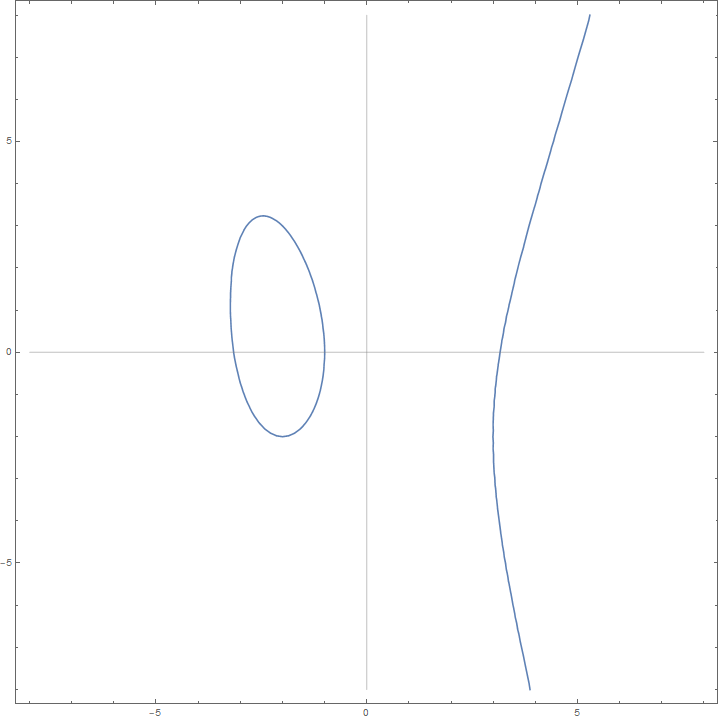
\includegraphics[scale=0.3]{figuras/eq_weierstrass}
  \caption{La curva real definida por la ecuación $y^2+xy+y=x^3+x^2-10x-10$.}
  \label{fig:eq_weierstrass}
\end{figure}%%%%%%%%%%%%%%%%%%%%%%%%%%%%%%%%%%%%%%%%%%%%%%%%%%%%%%%%%%%%%%%%%%%%%%%%%%
























Ahora estudiamos el grupo de puntos racionales de $X_0(15)$, que denotamos por $G=X_0(15)(\QQ)$. Por el profundo teorema de Mordell-Weil\footnote{Para toda curva elíptica $E$ sobre un campo numérico $K$, el grupo $E(K)$ es un grupo abeliano finitamente generado (cf. teorema 6.7 del capítulo VIII de \cite{SilvermanTAOEC}).} tenemos que
\[
	G\cong G_{\mathrm{tors}}\times\ZZ^r
\]
donde $G_{\mathrm{tors}}$ es el subgrupo de torsión y $r\geq0$ es el rango de $G$. Con esta descripción de $G$, nuestra tarea se divide en dos: estudiar el grupo de torsión y calcular el rango. El teorema de Nagell-Lutz lo vamos a usar para calcular 

\begin{prop}
  $\Gamma$ tiene 4 c\'uspides: $0,\tfrac{1}{3},\tfrac{1}{5},\tfrac{1}{15}$ (donde $\tfrac{1}{15}$
  es la c\'uspide $\infty$). No tiene puntos el\'ipticos y el g\'enero de $X$ es 1.
\end{prop}
\begin{proof}
  Todas las afirmaciones las probamos en el ejemplo \ref{ej:Gamma15} salvo la descripci\'on
  expl\'icitas de las c\'uspides. Sea $x/y\in\QQ$ expresado como fracci\'on irreducible, definimos
  $\delta=(15,y)$. Observe que $(\tfrac{15}{\delta},\tfrac{y}{\delta})=1$ y que
  $(x,\tfrac{y}{\delta})=1$ por hip\'otesis, entonces
  \[
    \exists c,d\in\ZZ \quad\text{tales que}\quad c\tfrac{15}{\delta}x+d\tfrac{y}{\delta}=1.
  \]
  En particular $(c,d)=1$.
  
  Por el teorema de Dirichlet sobre primos en progresiones aritm\'eticas\footnote{El
    teorema de Dirichlet dice que para cualesquiera
    $q$ y $n$ primos relativos, existen una infinidad de n\'umeros primos $p$ que satisfacen la
    congruencia $p\equiv q\Mod{n}$. Seguramente hay un argumento m\'as elemental para el caso particular
    de $\Gamma_0(15)$, pero el teorema de Dirichlet se puede generalizar f\'acilmente a cualquier
    $\Gamma_0(N)$.},
  podemos tomar $d$ un primo suficientemente gande y as\'i $(15,d)=1$. Por lo tanto $(15c,d)=1$
  y as\'i:
  \[
    \exists a,b\in\ZZ \quad\text{tales que}\quad ad-15bc=1.
  \]
  Por lo tanto obtenemos una matriz en $\Gamma$ y as\'i:
  \begin{align*}
    \frac{x}{y}
    &\equiv \mat{a}{b}{15c}{d}\frac{x}{y}=\frac{ax+by}{15cx+dy}
      =\frac{ax+by}{\delta(c\tfrac{15}{\delta}x+d\tfrac{y}{\delta})}
      =\frac{ax+by}{\delta}\Mod{\Gamma},\\
    \therefore\;\;\frac{x}{y}
    &\equiv\frac{x'}{\delta}\Mod{\Gamma}
      \quad\text{donde}\;\;\delta=(y,15)\;\;\text{y para alguna}\;\; x'\in\ZZ.   
  \end{align*}

  Podemos reducir el problema aun m\'as. Como $\Gamma$ contiene las matrices asociadas a las
  traslaciones $z\mapsto z+t$ por un entero $t$, tenemos que:  
  \begin{align*}
    \frac{x'}{\delta}
    &\equiv\mat{1}{-t}{0}{1}\frac{x'}{\delta}=\frac{x'-\delta t}{\delta}\Mod{\Gamma},\\
    \therefore\;\;\frac{x'}{\delta}
    &\equiv\frac{r}{\delta}\Mod{\Gamma}
      \quad\text{donde}\;\; 0\leq r<\delta.  
  \end{align*}
  Por lo tanto cada racional $x/y$ es congruente m\'odulo $\Gamma $a un racional en el
  siguiente conjunto
  \[
    \left\{\frac{0}{1},\frac{1}{3},\frac{2}{3},\frac{1}{5},\frac{2}{5},\frac{3}{5},\frac{4}{5},
      \frac{1}{15},\frac{2}{15},\frac{4}{15},\frac{7}{15},\frac{8}{15},\frac{11}{15},\frac{13}{15},
      \frac{14}{15}\right\}.
  \]
  Observa que si el denominador es $15$, entonces una fracci\'on irreducible $x/15$ induce una
  combinaci\'on lineal $ax+15b=1$ para algunas $a,b\in\ZZ$. Por lo tanto
  \[
    \frac{x}{15}\equiv \mat{a}{b}{-15}{x}\frac{x}{15}=\frac{ax-15b}{-15x+15x}=\infty \;\;\Mod{\Gamma}.
  \]
  Por lo tanto podemos reducir el conjunto de representantes: cada racional $x/y$ es congruente
  m\'odulo $\Gamma $a un racional en el siguiente conjunto
  \[
    \left\{0,\infty,\frac{1}{3},\frac{2}{3},\frac{1}{5},\frac{2}{5},\frac{3}{5},\frac{4}{5}\right\}.
  \]

  Observe que:
  \[
    \frac{1}{3}\equiv\mat{11}{-3}{15}{4}\frac{1}{3}=\frac{2}{3}\;\;\Mod{\Gamma}\quad\text{y}\quad
    \frac{1}{5}\equiv
    \begin{cases}
      \matt{7}{-1}{15}{-2}\frac{1}{5}=\frac{2}{5} \\
      \matt{-17}{4}{-30}{7}\frac{1}{5}=\frac{3}{5}\\
      \matt{11}{-3}{15}{-4}\frac{1}{5}=\frac{4}{5}
    \end{cases}\;\;\Mod{\Gamma}
  \]
  Por lo tanto cada racional $x/y$ es congruente m\'odulo $\Gamma$ a un racional en el siguiente
  conjunto
  \[
    \left\{0,\infty,\frac{1}{3},\frac{1}{5}\right\}.
  \]

  Afirmamos que este conjunto es el conjunto de c\'uspides de $\Gamma$. Debemos
  verificar que esos racionales son incongruentes dos a dos, peo aqu\'i solamente hacemos expl\'icitos
  dos relaciones porque las dem\'as son muy similares:
  \begin{align*}
 %   0\equiv\infty
 %   &\quad\then\quad \exists \gamma=\matt{a}{b}{15c}{d}\in\Gamma\;\;\text{tal que}\;\;
 %     \tfrac{1}{0}=\gamma\tfrac{0}{1}=\tfrac{b}{d}
 %   \quad\then\quad d=0\quad\then\quad 15\mid\det\gamma.\\
    0\equiv\frac{1}{3}
    &\quad\then\quad \exists \gamma=\matt{a}{b}{15c}{d}\in\Gamma\;\;\text{tal que}\;\;
      \tfrac{1}{3}=\gamma\tfrac{0}{1}=\tfrac{b}{d}
    \quad\then\quad d=3b\quad\then\quad 3\mid\det\gamma.\\
 %   0\equiv\frac{1}{5}
 %   &\quad\then\quad \exists \gamma=\matt{a}{b}{15c}{d}\in\Gamma\;\;\text{tal que}\;\;
 %     \tfrac{1}{5}=\gamma\tfrac{0}{1}=\tfrac{b}{d}
 %   \quad\then\quad d=5b\quad\then\quad 5\mid\det\gamma.\\
 %   \infty\equiv\frac{1}{3}
 %   &\quad\then\quad \exists \gamma=\matt{a}{b}{15c}{d}\in\Gamma\;\;\text{tal que}\;\;
 %     \tfrac{1}{3}=\gamma\tfrac{1}{0}=\tfrac{a}{15c}
 %     \quad\then\quad a=5c\quad\then\quad 5\mid\det\gamma.\\
 %   \infty\equiv\frac{1}{5}
 %   &\quad\then\quad \exists \gamma=\matt{a}{b}{15c}{d}\in\Gamma\;\;\text{tal que}\;\;
 %     \tfrac{1}{5}=\gamma\tfrac{1}{0}=\tfrac{a}{15c}
 %     \quad\then\quad a=3c\quad\then\quad 3\mid\det\gamma.\\
    \frac{1}{3}\equiv\frac{1}{5}
    &\quad\then\quad \exists \gamma=\matt{a}{b}{15c}{d}\in\Gamma\;\;\text{tal que}\;\;
      \tfrac{1}{5}=\gamma\tfrac{1}{3}=\tfrac{a+3b}{15c+3d}
      \quad\then\quad 3d=5a-15c+15d\\
    &\quad\then\quad 5\mid d\quad\then\quad 5\mid\det\gamma.
  \end{align*}
  Con esto terminamos la prueba.
\end{proof}

La figura \ref{fig:domfunGamma15} ilustra el dominio fundamental de $\Gamma$ y muestra sus
cuatro c\'uspides. Cada secci\'on del dominio fundamental es la traslaci\'on del dominio
fundamental de $\SL_2(\ZZ)$ por un representante de los elementos de $\SL_2(\ZZ)/\Gamma$
En el ap\'endice viene otra imagen del dominio fundamental donde cada secci\'on viene
etiquetada con la matriz q

\begin{figure}[!h]%%%%%%%%%%%%%%%%%%%%%%%%%%%%%%%%%%%%%%%%%%%% FIGURA
  \centering
  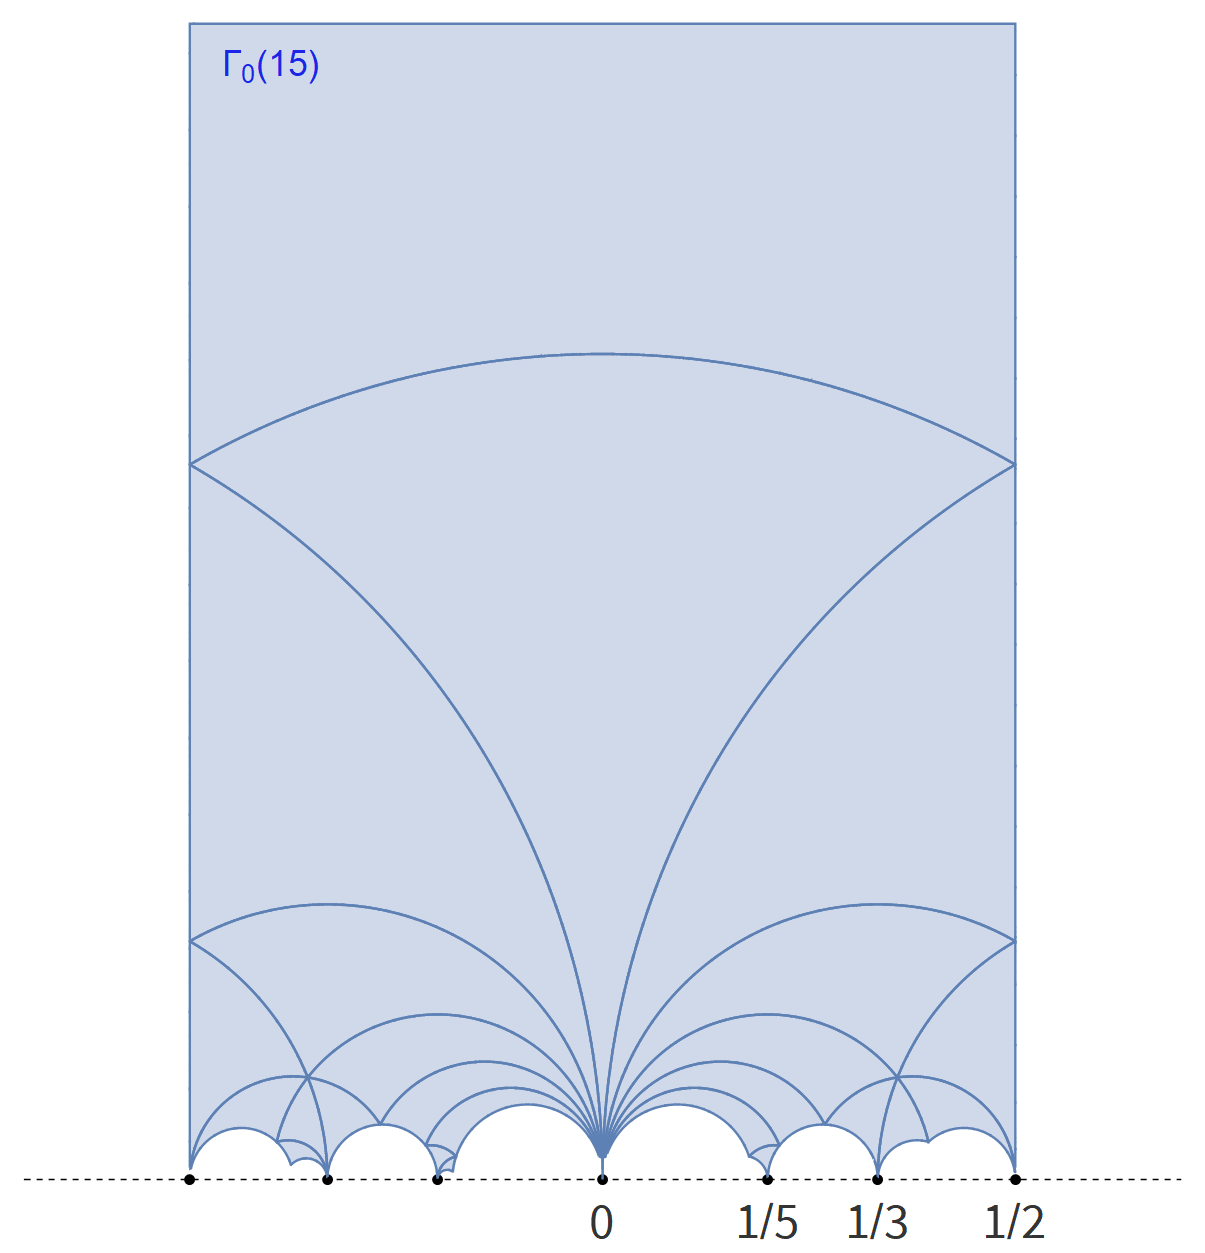
\includegraphics[scale=0.25]{figuras/domfundgamma015}
  \caption{El dominio fundamental del subgrupo de congruencia $\Gamma_0(15)$}
  \label{fig:domfunGamma15}
\end{figure}%%%%%%%%%%%%%%%%%%%%%%%%%%%%%%%%%%%%%%%%%%%%%%%%%%%%%%%%%%%%%%%%%%%%%%%%%%

Como $X$ es una cuva el\'iptica, el siguiente paso es calcular una ecuaci\'on de Weierstrass.
Este tema ha sido estudiado extensamente por Fricke \cite{Fricke}, Newmann \cite{NewmanCAAOACOMFII}
y resuelto por Ligozat \cite{LigozatCMDG1}, alumno de Ner\'on, en su tesis doctoral publicada por la
\emph{Soci\'et\'e math\'ematique de France}. Tenemos:

\begin{prop}
  La curva modular el\'iptica $X=X_0(15)$ tiene la ecuaci\'on de Weierstrass
  \[
    X:\;\; y^2+xy+y=x^3+x^2-10x-10
  \]
\end{prop}
\begin{proof}
  M\'as precisamente probamos que $X$ es isomorfo sobre $\QQ$ a la subvariedad proyectiva $W$
  definida por la ecuaci\'on homogenizada:
  \[
    y^2z+xyz+yz^2=x^3+x^2z-10xz^2-10z^3.
  \]
  Este hecho es esencialmente el Corolario 4.2.1 de \cite{LigozatCMDG1}, pero explicamos la prueba.
  Por Fricke (y en el caso general, por Newman) sabemos que la funci\'on
\end{proof}



. Los puntos racionales no-cuspidales de
la curva $X_0(15)$ corresponden a curvas el\'ipticas $E$ definidos sobre $\QQ$ tales que
$E(\overline{\QQ})$ contiene un subgrupo de orden 15 estable bajo la acci\'on natural
$G_{\QQ}\act E(\ol{\QQ})$. Los $j$-invariantes de esas curvas se pueden calcular y deducimos que
todas las curvas el\'ipticas asociadas a los puntos racionales no-cuspidales de $X_0(15)$ deben
ser modulares. En particular tendr\'iamos:

\begin{thm}\label{thm:subgrupoestable15}
  Si una curva el\'iptica $E$ sobre $\QQ$ es tal que $E(\overline{\QQ})$ contiene un subgrupo de
  orden 15 estable bajo la acci\'on de $G_{\QQ}$, entonces $E$ es modular.
\end{thm}

Para esto necesitamos
estudiar las propiedades geom\'etricas de $X_0(15)$.

En general, el grupo de congruencia $\Gamma_0(N)$ act\'ua sobre $\HH^*=\HH\cup\QQ\cup\{\infty\}$
mediante transformaciones de M\"obius y el espacio cociente $\HH^*/\Gamma_0(N)$ es una superficie
de Riemann compacta que denotamos por $X_0(N)$. Esta variedad tambi\'en se puede obtener
compactificando el espacio $\HH/\Gamma_0(N)$, agreg\'andole las c\'uspides de la acci\'on.

Para pobar el teorema \ref{thm:subgrupoestable15} necesitamos las siguientes propiedades de
$X_0(15)$ (cf. \cite[cap\'itulo XVI, \S 2, Lema 9]{CornellMFAFLT}):

\begin{prop}\label{prop:propiedadesx015}
  La curva modular $X_0(15)$ cumple las siguientes propiedades:
  \begin{enumerate}[label=\emph{\roman*})]
  \item $X_0(15)$ es una curva de g\'enero 1 con cuatro c\'uspides racionales.
  \item $X_0(15)$ tiene 8 puntos racionales, ie. $\# X_0(15)(\QQ)=8$.
  \item Los cuatro puntos racionales no-cuspidales de $X_0(15)(\QQ)$ corresponden a cuatro
    clases de isomorfismos de parejas $(E_i,C_i)$ donde $C_i\subset E_i(\overline{\QQ})$ es un
    subgrupo de orden 15 y cuyos $j$-invariantes son:
    \[
      j(E_i)\in\left\{
        -\frac{5^2}{2},-\frac{5^2241^3}{2^3},-\frac{5\cdot 29^3}{2^5},\frac{5\cdot 211^3}{2^{15}}
      \right\}
    \]
    
  \end{enumerate}
\end{prop}

\begin{proof}
  El g\'enero $g$ de $X_0(N)$ se calcula con la siguiente f\'ormula
  \cite[\S1.6, proposici\'on 1.40]{ShimuraITTATOAF}:
  \[
    g=1+\frac{\mu}{12}-\frac{\nu_2}{4}-\frac{\nu_3}{3}-\frac{\nu_{\infty}}{2}
  \]
  donde $\mu=[\PSL_2\ZZ:\overline{\Gamma}_0(N)]$ (aqu\'i $\overline{\Gamma}_0(N)$ es la imagen de
  $\Gamma_0(N)$ bajo la proyecci\'on $\SL_2\ZZ\epi\PSL_2\ZZ$), $\nu_2$ (respectivamente $\nu_3$) es
  la cantidad de clases de equivalencia (bajo la acci\'on de $\overline{\Gamma}_0(N)$) de los
  puntos el\'ipticos de orden 2 (respectivamente de orden 3) y $\nu_{\infty}$ es la cantidad de
  clases de equivalencias de puntos c\'uspidales.

  Para calcular $\mu$ observamos que la imagen de la funci\'on
  \[
    \Gamma_0(N) \lra \SL_2(\ZZ/N\ZZ) \quad\text{definido por}\quad
    \begin{pmatrix}a&b\\c&d\end{pmatrix} \mapsto
    \begin{pmatrix}a+N\ZZ&b+N\ZZ\\c+N\ZZ&d+N\ZZ\end{pmatrix}
  \]
  es el conjunto de matrices de $\SL_2(\ZZ/N\ZZ)$ de la forma:
  \[
    \begin{pmatrix} a+N\ZZ&b+N\ZZ\\0&a^{-1}+N\ZZ \end{pmatrix}.
  \]
  Hay $N$ posibles elecciones para tomar $b$ y $\varphi(N)$ posibilidades para $a$ (donde $\varphi$
  es la funci\'on de Euler). Por lo tanto el orden de la imagen de $\Gamma_0(N)$ es $N\varphi(N)$.

  Por otro lado, el kernel de la funci\'on es el \emph{subgrupo de congruencia principal de nivel}
  $N$:
  \[
    \Gamma(N):=\left\{
      \begin{pmatrix}a&b\\c&d\end{pmatrix}\in\SL_2\ZZ : a\equiv d\equiv 1,\; b\equiv c\equiv 0 \Mod{N}
    \right\}
  \]
  Adem\'as $\Gamma(N)$ se realiza como el kernel del homomorfismo $\SL_2\ZZ\ra\SL_2(\ZZ/N/ZZ)$. Por
  lo tanto $[\SL_2\ZZ:\Gamma(N)]$
\end{proof}

\subsection{Curvas modulares y espacios moduli}%%%%%%%%%%%%%%%%%%%%%%%%%%%%%%%%%%%%%%%%%%%%%%%%

En esta secci\'on definimos la curva $X_0(N)$ y vemos que parametriza ciertas clases de
isomorfismo de curvas el\'ipticas. Fijamos $N>1$.

Sea $E$ una curva el\'iptica sobre el campo $\QQ(x)$ tal que $j(E)=x$. Sea $P\in E$ un punto de
orden $n$ y sea $C=\{O,P,2P,\ldots,(N-1)P\}$ el subgrupo de $E$ generado por $P$. Toma
$K\subset\overline{\QQ(x)}$ como el campo fijo del subgrupo
$H=\{\sigma\in G_{\QQ(x)}\mid \sigma(C)=C\}$.

Como $(G_{\QQ(x)}:H)<\infty$ (porque $C$ es finito), entonces $K$ es una extensi\'on finita
de $\QQ(x)$. En particular es una extensi\'on de $\QQ$ finitamente generada. Ahora, si
$\overline{\QQ}\cap K=\QQ$ (estamos identificando a $\overline{\QQ}$ con su inclusi\'on en
$\overline{K}$) entonces $K$ es una extensi\'on de $\QQ$ finitamente generada de grado de
trascendencia 1. De esta manera, como la categor\'ia de curvas proyectivas suaves definidas
sobre $\QQ$ (con morfismos dominantes) y la categor\'ia de extensiones de $\QQ$ finitamente
generadas de grado de trascendencia 1 (cf. \cite[\S1.6, corolario 6.12]{HartshorneAG}), podemos
asociar a $K$ una curva proyectiva suave definida sobre $\QQ$ que llamamos $X_0(N)$.

Hay que probar que la elecci\'on de $X_0(N)$ est\'a bien definida, es decir que no depende de
$E$ ni de el subgrupo $C\subset E$ y adem\'as que efectivamente $\overline{\QQ}\cap K=\QQ$ para que
$K$ realmente sea un campo de funciones de una curva. Estas tres proposiciones se siguen del
siguiente teorema:

Sea $E$ una curva el\'iptica sobre $\QQ$ y definimos a $\QQ(E[N])$ como la extensi\'on de
Galois generada por las coordenadas afines de los puntos de $E[N]$. La acci\'on natural
$G_{\QQ(E[N])}\curvearrowright E[N]$ induce una representaci\'on
$\rho:G_{\QQ(E[N])}\ra\GL_{2}(\ZZ/N\ZZ)$ (gracias a la estructura de $E[N]$ dada en la proposici\'on
\ref{prop:estructura_EN}).

\begin{thm}\label{thm:iso_gruposgalois}
  Sea $E$ una curva el\'iptica definida sobre $k=\QQ(x)$ tal que $j(E)=x$. Con la notaci\'on del
  p\'arrafo anterior, la representaci\'on $\rho$ es un isomorfismo, es decir:
  \[
    G_{\QQ(x,E[N])}\cong\GL_{2}(\ZZ/N\ZZ).
  \]
  Adem\'as, $\overline{\QQ}\cap\QQ(x,E[N])=\QQ(\mu_N)$ donde $\mu_N\subset\CC$
  es el conjunto de las $N$-\'esimas raices de la unidad.
\end{thm}

\begin{nota}
  Este resultado es una versi\'on d\'ebil del caso $k=\CC(x)$ donde el isomorfismo es
  $\Gal(\QQ(x,E[N])\mid\QQ(x))\cong\SL_{2}(\ZZ/N\ZZ)$ (cf.
  \cite[cap\'itulo III, \S1, teorema 1 y su corolario]{CornellMFAFLT})
\end{nota}

Ahora explicamos porque la elecci\'on $X_0(N)$ est\'a bien definida:

\begin{cor}
  La curva el\'iptica $X_0(N)$ sobre $\QQ$ existe y no depende de $E$ ni del subgrupo $C$.
\end{cor}

\begin{proof}
  Como mencionamos antes, basta robar que $\overline{\QQ}\cap K=\QQ$ para que $K$ efectivamente
  sea una extensi\'on finitamente generada sobre $\QQ$ de grado de trascendencia 1. Sea $P\in E$
  el generador de $C$. Observa que $\{P\}\subset E[N]$ se puede extender a una base ordenada de
  tal manera que el isomorfismo $G_{\QQ(x,E[N])}\cong\GL_2(\ZZ/N\ZZ)$ del teorema
  \ref{thm:iso_gruposgalois} hace que $H':=\{\sigma\in G_{\QQ(x,E[N])}\mid \sigma(C)=C\}$ sea
  isomorfo a las matrices triangulares inferiores, i.e.
  \[
    H\cong\left\{ \begin{pmatrix}a&0\\b&d\end{pmatrix}:a,d\in(\ZZ/N\ZZ)^{*},\; b\in\ZZ/N\ZZ\right\}.
  \]
  
  Ahora, la funci\'on determinante $\det:\GL_2(\ZZ/N\ZZ)\ra(\ZZ/N\ZZ)^*$ restringida a $H$ sigue
  siendo sobre. Por lo tanto $\QQ(\mu_N)\cap K=\QQ$....
  Si sustituimos la igualdad de la segunda parte del teorema \ref{thm:iso_gruposgalois} en esta
  f\'ormula obtenemos:
  \[
    \QQ=
    \Big(\overline{\QQ}\cap\QQ(x,E[N])\Big)\cap K=
    \QQ(x,E[N])\cap \big(\overline{\QQ}\cap K\big)=\overline{\QQ}\cap K
  \]
  ya que $\overline{\QQ}\cap K\subset\QQ(x,E[N])$.

  Ahora probamos que $X_0(N)$ es independiente de la elecci\'on de $C$. Cambiar de subgrupo $C$ es
  cambiar de punto $P$ de orden $N$. Sean $P'\in E$ otro punto de orden $N$, $C'\subset E[N]$ el
  subgrupo c\'iclico generado por $P'$ y $H'$ el subgrupo de $G_{\QQ(x,E[N])}$ de fija a $C'$. De la
  misma manera extendemos $\{P'\}$ a otra base de $E[N]$. Este cambio de base modifica el
  isomorfismo $G_{\QQ(x,E[N])}\cong\GL_2(\ZZ/N\ZZ)$ mediante una conjugaci\'on por la matriz de cambio
  de base. En particular la imagen de $H'$ en $\GL_2(\ZZ/N\ZZ)$ es un conjugado de la imagen de $H$.
  Por lo tanto existe un $\sigma\in G_{\QQ(x,E[N])}$ tal que $H'=\sigma H\sigma^{-1}$. Por lo tanto
  el campo fijo $K'$ de $H'$ es simplemente $\sigma(K)$, es decir $K\cong K'$. Gracias a la
  equivalencia de categor\'ias mencionada al principio de la secci\'on, $X_0(N)$ es isomorfo a
  cualquier curva proyectiva suave con campo de funciones $K'$ y por lo tanto $X_0(N)$ es
  independiente de la elecci\'on de $C$.

  Por \'ultimo probamos que $X_0(N)$ es independiente de la elecci\'on de la curva $E/\QQ(x)$....  
\end{proof}

Como consecuencia de este corolario, cada curva proyectiva $X_0(N)$ sobre $\QQ$ tiene asociado una
curva el\'iptica $E/\QQ(x)$ (con $j(E)=x$) y un subgrupo c\'iclico $C\subset E$ de orden $N$ tal que
el campo de funciones $K$ de $X_0(N)$ es el campo fijo de $H=\{\sigma\in G_{\QQ(x)}\mid \sigma(C)=C\}$.
La inclusi\'on $\QQ(x)\hookrightarrow K$ induce un morfismo de curvas $X_0(N)\ra\PP^1(\QQ)$. 
A un punto en la imagen inversa de $\infty\in\PP^1(\QQ)$ se le llama una \emph{c\'uspide} de
$X_0(N)$.

Tambi\'en podemos considerar a $X_0(N)$ como una curva proyectiva sobre $\CC$; en este caso su
campo de funciones es $K\otimes_{\QQ}\CC$. Como en el p\'arrafo anterior, la inclusi\'on
$\CC(x)\hookrightarrow K\otimes\CC$  determina un morfismo $X_0(N)(\CC)\ra\PP^1(\CC)$. Sea
$S\subseteq\PP^1(\CC)$ un subconjunto y $S^{\text{c}}$ su complemento en $\PP^1(\CC)$. Denotamos
$X_0(N)(\CC)_S$ como la imagen inversa de $S^{\text{c}}$ bajo $X_0(N)(\CC)\ra\PP^1(\CC)$.

Estamos en posici\'on de estudiar c\'omo parametriza $X_0(N)$ a algunas curvas el\'ipticas, pero
primero debemos definir una categor\'ia nueva. Los objetos son parejas $(E,C)$ donde $E/\CC$ es
una curva el\'iptica y $C\subset E$ es un subgrupo c\'iclico de orden $N$. Los morfismos
$(E,C)\ra(E',C')$ son isomorfismos de curvas $\varphi:E\ra E'$ tales que $\varphi(C)=C'$. A la
clase de isomofismo de $(E,C)$ la denotamos por $[E,C]$ y al conjunto de clases de isomorfismo
lo denotamos por $\text{El}_0(N)(\CC)$. Adem\'as, si $S\subseteq\PP^1(\CC)$ entonces escribimos
\[
  \text{El}_0(N)(\CC)_S:=\{[E,C]\in\mathrm{El}_0(N)(\CC)\mid j(E)\not\in S\}.
\]
Similarmente denotamos por $\mathrm{Toro}_0(N)$ al conjunto de clases de isomorfismo de parejas
$(T,C)$ donde $T$ es un toro complejo de dimensi\'on 1 (i.e. $T\cong\CC/\Lambda$ para alguna ret\'icula)
y $C\subset T$ es un subgrupo c\'iclico de orden $N$.


Ahora, sea $x\in X_0(N)(\CC)$. Como $X_0(N)(\CC)$ es una curva suave, $x$ determina un anillo de
valoraci\'on discreta $\Oo_x\subset K\otimes\CC$ con ideal maximal $\m_x$. Si $E$ tiene buena
reducci\'on en $\m_x$, entonces la reducci\'on m\'odulo $\m_x$ produce una curva el\'iptica
$E_x/\CC$. La restricci\'on de la reducci\'on m\'odulo $\m_x$ a $E[n]\ra E_x[N]$ es inyectiva y
as\'i la reducci\'on m\'odulo $\m_x$ del punto $P\in E[N]$ es un punto $P_x\in E_x[N]$ de orden
$N$ que genera un subgrupo c\'iclico $C_x\subset E_x$ de orden $N$.

Con estas consideraciones podemos enunciar el resultado m\'as importante de esta secci\'on:
\begin{thm}
  Sean $E/\QQ(x)$ una curva el\'iptica tal que $j(E)=x$, $S\subseteq\PP^1(\CC)$ un subconjunto
  que contiene a todos los lugares donde $E$ tiene mala reducci\'on, $\{Q,P\}$ una $\ZZ/N\ZZ$-base
  de $E[N]$ y $C\subset E$ el subgrupo c\'iclico generado por $P$, entonces tenemos el siguiente
  diagrama conmutativo de funciones biyectivas:
  \[
    \begin{tikzcd}[column sep=large, row sep=large]
      X_0(N)(\CC)_S \arrow[r,"(i)"] \arrow[d,"(ii)"'] &
      \mathrm{El}_0(N)(\CC)_S \arrow[d,"(iv)"] \\
      \HH/\Gamma_0(N) \arrow[r,"(iii)"'] & \mathrm{Toro}_0(N)
    \end{tikzcd}
  \]
  donde las funciones est\'an dadas por:
  \begin{enumerate}[label=\emph{\roman*})]
  \item $x\mapsto [E_x,C_x]$.
  \item La restricci\'on del isomorfismo $X_0(N)(\CC)\cong\HH^*/\Gamma_0(N)$ de superficies de
    Riemann.
  \item $[z]\mapsto [\CC/\Lambda_z,\gen{\tfrac{1}{N}+\Lambda_z}]$ donde $\Lambda_z:=z\ZZ\oplus\ZZ$
    es una ret\'icula de $\CC$.
  \item $[E,C]\mapsto [E(\CC),C]$.
  \end{enumerate}
\end{thm}

\begin{proof}
  La prueba de que ($i$) es biyectiva se sigue de
  \cite[cap\'itulo III, \S1.3, proposici\'on 1]{CornellMFAFLT}, la biyectividad de ($ii$) se sigue
  de \cite[cap\'itulo III, \S1.10, proposici\'on 6]{CornellMFAFLT}, la biyectividad de ($iii$) se
  sigue de \cite[cap\'itulo III, \S1.10, proposici\'on 7]{CornellMFAFLT} y la biyectividad de
  ($iv$) se sigue de \cite[cap\'itulo III, \S1.8, proposici\'on 5]{CornellMFAFLT}.
\end{proof}

\begin{defin}
  Una curva el\'iptica $E/\QQ$ es \emph{modular} si existe una funci\'on holomorfa no constante
  $X_0(N)\ra E$ para alguna $N$.
\end{defin}


\end{document}
